\documentclass[times, utf8, seminar, numeric]{fer}
\usepackage{booktabs}
\usepackage{algorithm}
\usepackage{algpseudocode}
\usepackage{amssymb}
\usepackage{amsmath}
\usepackage{bm}
\usepackage{graphicx}
\usepackage{subfig}
\usepackage{hyperref}
\usepackage{listings}

\graphicspath{ {./images/} }

\DeclareMathOperator*{\argmax}{arg\,max}
\DeclareMathOperator*{\argmin}{arg\,min}

\algnewcommand\algorithmicforeach{\textbf{for each}}
\algdef{S}[FOR]{ForEach}[1]{\algorithmicforeach\ #1\ \algorithmicdo}

\newcommand{\eng}[1]{(engl. \textsl{#1}\/)}
\newcommand{\vect}[1]{\bm{\mathrm{#1}}}

\def\todo#1{\fbox{\begin{minipage}{30em}
      {\bf TODO: } #1
\end{minipage}}}

\renewcommand{\lstlistingname}{Isječak koda}


\begin{document}



\nocite{*}

\title{Uklanjanje šuma na slikama iscrtanim Monte Carlo
metodama primjenom dubokih konvolucijskih modela}

\author{Nikola Bunjevac}

\voditelj{prof. dr. sc. Siniša Šegvić}

\maketitle

\tableofcontents

\chapter{Uvod}
Računalna grafika vrlo je široko i zanimljivo područje računarstva. Ona se bavi izradom vizualnih
reprezentacija (slika, video...) iz ostalih načina zapisa u računalu. Primjerice, možemo imati
opis scene u tekstualnoj datoteci koju će zatim iscrtavatelj \engl{renderer} pročitati i iscrtati
prikaz te scene na ekranu.

Prije nego počne iscrtavanje, program prvo mora pročitati i \textit{parsirati} datoteku u kojoj
je pohranjen opis scene. Postoji mnogo načina reprezentacije scene i objekata koji se u njoj
nalaze. Najčešće je korišten prikaz pomoću poligona, točnije trokuta. Osim pozicija vrhova,
svaki objekt ima još neka svojstva kao što su materijali, transformacije, itd. Osim objekata,
potrebni su nam još podaci o virtualnoj kameri i osvjetljenju kako bismo mogli iscrtati prikaz.
Nakon učitavanja navedenih informacija, obično se izgrađuju strukture za ubrzavanje rada, poput
hijerarhija obujmica \engl{bounding volume hierarchies, BVH} koje služe za brzo određivanje
presjecišta u sceni. Nakon što su učitane sve potrebne informacije i obavljene sve predradnje,
može početi postupak iscrtavanja.

Postoje razne tehnike za iscrtavanje scena, a među češće korištenima su rasterizacija i
praćenje zrake \eng{raytracing}. Uobičajeno, grafičke kartice (GPU) koriste rasterizaciju, dok
se praćenje zrake obično izvodi na procesoru (CPU), iako se i taj trend postupno mijenja.

Prirodno bismo očekivali precizan prikaz scene na ekranu, no iz iskustva znamo da to nije uvijek
tako. Ako se dovoljno približimo zaslonu računala, vidjet ćemo male točkice koje zovemo pikselima.
Matematički opis scene koji koristi dvodimenzionalne točke povezane raznim funkcijama nazivamo
vektorskom grafikom.
Rasterizacija je postupak pretvorbe iz vektorske grafike u rasterski prikaz--niz piksela, točaka
ili linija koji zajedno na zaslonu tvore sliku. Ovdje je važno primijetiti kako se rasterska
slika sastoji od diskretnih elemenata, dok se vektorski zapis ne sastoji. To je razlog zašto
ne možemo uvijek prikazati sve oštro na zaslonu. Primjerice, sliku u vektorskom zapisu možemo
zumirati proizvoljno, bez gubitka kvalitete, dok će ista operacija na rasterskoj slici dovesti
do toga da ćemo vidjeti pojedine piksele i izgubiti detalje slike.

Drugi važan postupak jest praćenje zrake. To je također postupak stvaranja slike
koju možemo prikazati na zaslonu, ali na drugačiji način. U ovom slučaju ćemo za svaki piksel
slike ``ispucati'' zraku iz kamere i pratiti njenu interakciju s površinama u trodimenzionalnoj
sceni. Time ćemo dobiti niz piksela, kao kod rasterizacije, koji ponovo tvore sliku koju možemo
prikazati.

Važan pojam je i fotorealistično iscrtavanje koje za cilj ima generirati prikaz scene koji ne
možemo razlikovati od fotografije uslikane fotoaparatom koja bi prikazivala istu takvu scenu
u stvarnom svijetu. Naravno, teško je scenu iz stvarnog svijeta opisati u računalu, ali
ostvaren je značajan napredak na tom području.

Postupak rasterizacije se obično koristi za interaktivnu računalnu grafiku koja se prikazuje u
stvarnom vremenu, dok se praćenje zrake koristi za neinteraktivno iscrtavanje \engl{offline
  rendering}. U ostatku dokumentacije ćemo se usredotočiti na postupak praćenja zrake i
fotorealistično iscrtavanje.

Kako je postupak praćenja zrake vrlo računalno zahtjevan, postoje mnogi pokušaji ubrzavanja tog
postupka. Neki se koriste kao komplementarni, dok se neki koriste zasebno.

Donedavno najbolji postupci nisu koristili metode strojnog, tj. dubokog učenja. Jedan od razloga
je što takve metode nisu bile široko raširene, a osim toga, nisu bile računalno traktabilne. One
također zahtijevaju veliku količinu podataka kako bi donijele željene rezultate što dodatno
otežava problem. Ipak, u posljednjih nekoliko godina korištenje dubokog učenja postalo je sve
pristupačnije pa je samim time stiglo i do računalne grafike. Možemo reći kako se takvi postupci
nadograđuju na prethodne (``klasične''), samo što su fleksibilniji od njih jer se prilagođavaju
podacima. Drugim riječima, učenje nad velikom količinom podataka omogućuje nam da ostvarimo
generalizaciju nad raznim podacima i uvjetima.

Učenje nad označenim podacima (u našem slučaju parovima šumovitih i referentnih slika) naziva
se nadzirano učenje \eng{supervised learning}.

Još jedan važan pojam koji ćemo koristiti su duboki konvolucijski modeli. Oni se
sastoje od niza slojeva koje nazivamo konvolucijskim slojevima. Svaki sloj sadrži jezgre koje
se primjenjuju na ulaz u sloj i time dobivamo određeni izlaz koji nazivamo mapama značajki.
Svaka jezgra ima težine, a dodatno može imati i pomak \engl{bias}.
Uobičajeno nakon svakog konvolucijskog sloja slijede slojevi sažimanja i aktivacijska funkcija.

Jedna od prednosti takvih modela je velika prilagodljivost, neovisnost o veličini ulaza (što je
vrlo korisno kod slika), manji broj parametara od alternativa, itd.

Sljedeći pojam koji smo spomenuli su parametri. Oni su predmet učenja modela strojnog učenja,
odnosno njih možemo mijenjati i prilagođavati kako obrađujemo podatke za učenje. Kod
konvolucijskih slojeva možemo učiti težine i pomak svake jezgre.


\section{Monte Carlo integracija}
Korištenje Monte Carlo metoda\footnote{\url{https://en.wikipedia.org/wiki/Monte_Carlo_method}} se
u posljednje vrijeme pokazalo kao vrlo pogodnim rješenjem problema iscrtavanja. Takve metode se
temelje na korištenju nasumično generiranih brojeva kako bi aproksimirale krajnji numerički
rezultat.

Iscrtavanje se temelji na rješavanju jednadžbe iscrtavanja koja se još naziva i jednadžbe širenja
svjetlosti \eng{rendering equation, light transport equation}
\begin{equation} \label{eq:1}
  L_o(\vect{p}, \vect{\omega_o}) = L_e(\vect{p}, \vect{\omega_o}) + \int_{S^2} f(\vect{p}, \vect{\omega_o}, \vect{\omega_i})
  L_i(\vect{p}, \vect{\omega_i}) |\cos\theta_i| \mathrm{d}\vect{\omega_i}.
  \end{equation}
Pomoću nje računamo izlazno osvjetljenje $L_o(\vect{p}, \vect{\omega_o})$ u točki prostora $\vect{p}$ u smjeru $\vect{\omega_o}$. Ono se sastoji od dvije komponente:
emitirane svjetlosti $L_e(\vect{p}, \vect{\omega_o})$ te utjecaja sporedne
svjetlosti iz svih smjerova kugle $S^3$ oko točke $\vect{p}$ skalirane
funkcijom $f(\vect{p}, \vect{\omega_o}, \vect{\omega_i})$ i kosinusom kuta između $\vect{\omega_o}$ i $\vect{\omega_i}$ \cite{pbrbook}.

Navedena jednadžba iznimno je zahtjevna za rješavanje te nema analitičko
rješenje, osim za najjednostavnije slučajeve.
Postoje mnoge metode za numeričku aproksimaciju integrala, ali one funkcioniraju dobro samo za
integrale niske dimenzionalnosti. Ako imamo više dimenzija,
rezultati više nisu zadovoljivi.

Stoga pribjegavamo metodi
Monte Carlo aproksimacije integrala \cite{pbrbook}. Pravilna primjena te metode daje odlične rezultate i to ju čini jednom od metoda
koja daje rezultat najbliži fizikalno ispravnom rezultatu koji bismo dobili kao analitičko rješenje gornjeg integrala.

Korisnost Monte Carlo aproksimacije integrala leži u svojstvu da koristeći nasumičnost za
evaluaciju integrala čine stopu konvergencije neovisnu o broju dimenzija. Još jedna prednost
je što ova metoda zahtijeva samo mogućnost evaluacije funkcije na nasumičnim pozicijama, tj.
funkciju možemo predstaviti crnom kutijom koja za dani ulaz daje pripadajući izlaz. Ne moramo
znati kako crna kutija funkcionira iznutra.

Kako bismo dobili procjenu integrala pomoću ovog algoritma, potrebno je provesti dovoljan broj
uzorkovanja i uprosječiti dobivene rezultate. Očekivanje ove procjene je jednako točnoj
vrijednosti integrala \cite{pbrbook}.

Spomenimo još i Las Vegas metode koje također koriste nasumične brojeve. Razlika između ovih dviju metoda je što Las Vegas metode mogu ``različitim putevima'' doći uvijek do istog rješenja, dok Monte Carlo metode ne moraju
uvijek dati isto rješenje.


\section{Uzorkovanje}
Postupak praćenja zrake uvelike ovisi o količini uzorkovanja svakog piksela, tj. jednadžbe \ref{eq:1}.
Nakon što ispucamo
zraku iz kamere, pratimo gdje će se ona odbiti, te pratimo izvore svjetlosti i utjecaj okoline.
Ako uzorkujemo uniformno u svim smjerovima, rezultati neće biti zadovoljavajući. Stoga su
razvijene metode koje favoriziraju “teške” situacije, odnosno bolje je da vrijeme utrošimo na
uzorkovanje u smjerovima bliže izvorima svjetlosti, područjima koja se nalaze u sjeni, rubovima
površina itd.

Naravno, što više uzoraka po pikselu imamo, to će rezultat biti bolji, ali će i vrijeme izračuna
biti veće. Savršeno iscrtavanje dobivamo kada broj uzoraka teži u beskonačnost. Stoga, željeli
bismo izbjeći veliku količinu uzorkovanja.

\begin{figure}[h]
\centering
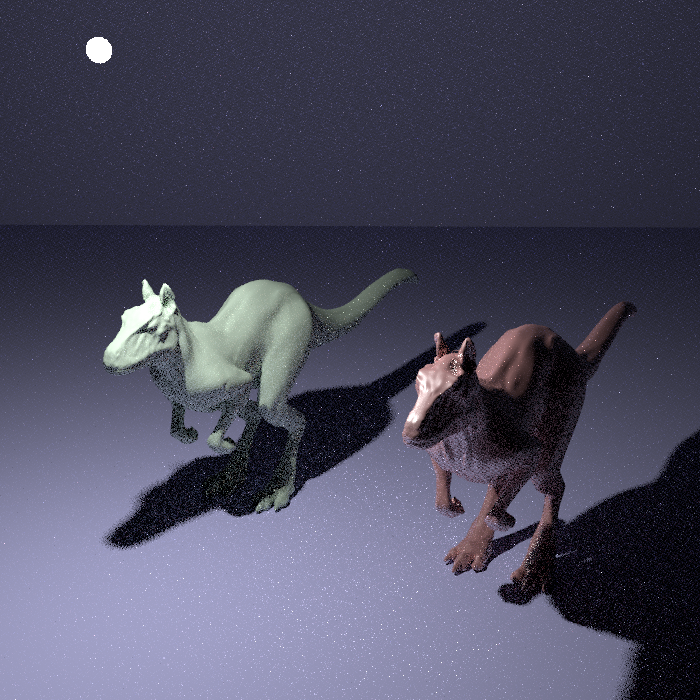
\includegraphics[width=0.5\textwidth]{killeroo4.png}
\caption{Primjer šuma pri malom broju uzoraka. Slika je dobivena iscrtavateljem \textit{pbrt}\protect\footnotemark s 4 uzorka po pikselu.}
\label{fig:killeroo}
\end{figure}

\footnotetext{\url{https://www.pbrt.org/}}

Problem koji se javlja pri malom broju uzoraka je šum koji prikazuje \ref{fig:killeroo}. Možemo
primijetiti kako se on pogotovo ističe na područjima u sjeni i rubovima. To nam daje naznaku
da ćemo se morati posebno usredotočiti na takva područja.

Ono što bismo htjeli postići jest da sa što manje uzoraka imamo što bolji rezultat.
Kako bismo to postigli, iscrtat ćemo sliku s malim brojem uzoraka te na takvoj slici pokušati
otkloniti šum.



\chapter{Teorijska podloga}
Prvo ćemo opisati teoretsku podlogu problema. Označimo piksel $p$ kao $\mathbf{x_p}$. Tada
svaki piksel možemo prikazati kao
$$\vect{x_p} = \{\vect{c_p}, \vect{f_p}\}, \quad \vect{x_p} \in \mathbb{R}^{3+D},$$
pri čemu je $\vect{c_p}$ boja u RGB zapisu, a $\vect{f_p}$ vektor $D$ dodatnih značajki.

RGB zapis se sastoji od 3 boje - crvene, zelene i plave. Takav način zapisa je praktičan i univerzalno
rasprostranjen. Važno je napomenuti kako su vrijednosti u RGB zapisu koje možemo prikazati na ekranu u rasponu $[0, 1]$, ali izlaz
iz iscrtavatelja nije ograničen navedenim rasponom. Ostale značajke također ne moraju biti u tom rasponu, primjerice dubina.

Dodatne značajke koje želimo izvući iz iscrtavatelja osim boje su:
\begin{itemize}
\item normale,
\item dubina,
\item albedo.
\end{itemize}

Normale predstavljaju vektore okomite na površinu u točki najbližeg presjecišta zrake iz kamere i površine.
Značajka dubine pohranjuje udaljenost od kamere do najbližeg presjecišta. Albedo predstavlja boje teksture
bez primijenjenog osvjetljenja. Drugim riječima, difuznu komponentu možemo
prikazati kao umnožak albeda i efektivnog osvjetljenja \engl{effective irradiance}
\cite{vogels2016thesis}.

Referentnu boju piksela označimo s $\vect{\bar{c}_p}$. Savršenu referentnu boju ne možemo
izračunati jer bismo trebali beskonačan broj uzoraka, ali u praksi je dovoljno da broj uzoraka
bude velik (u skupu podataka on iznosi $8192$). Tada želimo na temelju ulaznog piksela pronaći
procjenu boje koju ćemo označiti s $\vect{\tilde{c}_p}$.

Kako bismo postigli što bolju procjenu, obično to ne radimo na temelju samo jednog piksela, već
na temelju piksela i njegova susjedstva $\mathrm{N}(\vect{p})$. Blok vektora (boje i značajke)
pridruženih pikselima u susjedstvu od $\vect{p}$ označimo s $\vect{X_p}$.

Želimo pronaći funkciju $g(\vect{X_p}; \bm{\theta})=\vect{\hat{c}_p}$ koja će na temelju bloka
piksela $\vect{X_p}$ i parametara $\bm{\theta}$ procijeniti vrijednost boje piksela s uklonjenim
šumom. Ta funkcija, odnosno njezini parametri, su središnji pojam problema uklanjanja šuma.

Rješenje problema pronalaska takve funkcije možemo definirati kao
$$ \vect{\hat{\theta}_p} = \argmin_{\bm{\theta}} l(\vect{\bar{c}_p}, g(\vect{X_p}; \bm{\theta})), $$
gdje je $l(\vect{\bar{c}}, \vect{\hat{c}})$ funkcija gubitka između referentne boje i procjene.
No, tu se javlja problem jer nemamo $\vect{\bar{c}_p}$, tj. referentnu boju piksela.

Većina metoda za uklanjanje (Monte Carlo) šuma, mijenjaju
funkciju $g$ transformacijom $\bm{\theta}^\intercal\phi(\vect{x_q})$, gdje je $\phi: \mathbb{R}^{3+D}
\to \mathbb{R}^{M}$. Nakon toga metodom najmanjih kvadrata rješavaju težinsku regresiju
$$ \sum_{\vect{q} \in \mathrm{N(\vect{p})}}(\vect{c_q} - \vect{\theta}^\intercal\phi(\vect{x_q}))^2
\omega(\vect{x_p}, \vect{x_q}), $$
gdje $\omega$ nazivamo jezgrom ili filtrom. Intuitivno, ona pomaže u razlučivanju između piksela
koji su šum i treba im dati manju važnost i onih ispravnih koje želimo više uvažiti.

Problem koji se javlja kod takvih metoda je odabir filtra. On je fiksan i ne nudi fleksibilnost, a
mora davati dobre rezultate za vrlo širok spektar ulaznih podataka. Jedno moguće poboljšanje je
primijeniti regresiju većega stupnja čime ćemo dobiti i bolji rezultat, ali to nerijetko dovodi
do prevelike prilagodbe podacima \engl{overfitting}.

To nas dovodi do ideje da primijenimo metode dubokog učenja. Za to nam je potreban skup podataka
za učenje koji će biti centralni pojam ove metode. Označimo ga s $\mathcal{D}$. Kako ćemo
koristiti nadzirano učenje, $\mathcal{D}$ će se sastojati od $N$ parova primjera za učenje i
pripadne referentne boje piksela. To možemo zapisati kao
$$ \mathcal{D} = \{ (\vect{X}_1, \vect{\bar{c}}_1), \ldots, (\vect{X}_N, \vect{\bar{c}}_N) \}. $$

U našem slučaju ćemo imati sličice \engl{patch} veličine $65\times65$ piksela dobivene iz većih
slika iscrtanih Monte Carlo metodama. Ulazna sličica će imati manji broj uzoraka, dok će
referentna sličica iz skupa za učenje imati velik broj uzoraka. Cilj nam je ukloniti šum na
ulaznoj sličici i dobiti rezultat što sličniji referentnoj.

\chapter{Skup podataka za učenje}
Sada ćemo se pozabaviti analizom skupa podataka \engl{dataset}. On je javno dostupan na službenoj
stranici članka\footnote{\url{http://drz.disneyresearch.com/~jnovak/publications/KPCN/}}. Kako
se radi o slikama koje osim RGB boje imaju i niz dodatnih značajki, veličina skupa je očekivano
zavidna, gotovo 300 GiB.

\section{Iscrtavanje scena}
Skup se sastoji od 1482 nasumične permutacije 8 javno dostupnih scena. Kako je 8 scena relativno
mala količina podataka za potrebe metode, umjetno su generirane dodatne scene tako da su se
parametri scene nasumično mijenjali iz unaprijed zadanog skupa vrijednosti. Tako dobivene scene
iscrtane su modificiranim iscrtavateljem \textit{Tungsten}\/
\footnote{\url{https://github.com/tunabrain/tungsten}} (modificirana verzija je dostupna na
stranici članka). Razlog modifikacije je što željene dodatne značajke koje koristimo pri učenju
uobičajeno nisu dio standardnog izlaza pa ih je bilo potrebno dodati.

Kao što smo napomenuli, scene su dobivene permutacijom izvornih 8 scena. Permutirane značajke su
\begin{itemize}
\item mapa okoline (rotiranje) i položaj sunca,
\item hrapavost materijala \engl{roughness},
\item teksture unutar pripadnog razreda (npr. pod, tapete, kamen, drvo, \ldots),
\item jačina svjetlosti,
\item kamera.
\end{itemize}
Značajke kamere su permutirane tako da su određene točke interesa u sceni u koje kamera
gleda, a zatim se kamera pomicala unutar određenog prostora. Širina pogleda \engl{field of view}
je također mijenjana, a korištene su i dvije vrste kamere—jednostavna kamera \engl{pinhole camera}
te kamera s tankom lećom. Permutacije scene koje nakon iscrtavanja nisu imale značaja,
primjerice, bile su potpuno crne, su ručno izbačene. Iscrtane slike pohranjene su u EXR formatu
koji podržava visoki raspon vrijednosti i više kanala u slici što je praktično za pohranu
dodatnih značajki izlaza.

Razlog permutiranja scena jest postizanje što veće raznolikosti kako bi se izbjegla prenaučenost.
Druga mogućnost je bila izraditi veliki broj različitih scena, međutim, to nije izvedivo iz više
razloga - cijene, vremena, ljudi, itd.

Kako bismo imali parove za učenje, slike su iscrtane u više razina uzorkovanja, u potencijama
broja 2, od 128 do 1024 uzorka za šumovite slike, te 8192 uzorka za referentne slike. Najviše
uzorkovane slike ipak nisu savršene, ali izlaz je dovoljno konvergirao kako bismo ih mogli
proglasiti referentnima. Slike s prisutnim šumom su izlaz jednog pokretanja iscrtavatelja, dok je
referenca iscrtana posebno kako bi se dobio neovisan rezultat (drukčiji \textit{seed} generatora
nasumičnih brojeva).

\section{Značajke izlaznih slika}
Generirane slike su veličine $1280\times720$ piksela i pohranjene su u EXR formatu. Već smo
spomenuli kako iscrtane slike osim glavnog RGB kanala (ali ne ograničenog na interval [0, 1], već
visokog raspona \engl{high dynamic range, HDR}) sadrže i dodatne značajke koje ćemo koristiti u
učenju modela. Značajke svake EXR datoteke su (pojašnjenja u nastavku)
\begin{itemize}
\item RGB boja (glavni kanal, 3 komponente),
\item difuzni kanal (3 komponente),
\item zrcalni kanal (3 komponente),
\item albedo (3 komponente),
\item dubina (1 komponenta),
\item normale (3 komponente),
\item vidljivost izvora svjetlosti (1 komponenta).
\end{itemize}

RGB boja se može podijeliti na difuzni i zrcalni kanal (zbroj). Nadalje, difuzni kanal se može
podijeliti na albedo i efektivno osvjetljenje (umnožak). Albedo predstavlja boju teksture bez
osvjetljenja. Dubina predstavlja udaljenost od kamere prvog presjecišta zrake. Normale su vektori
okomiti na površinu u točki najbližeg sjecišta zrake iz kamere. Na prvom presjecištu također
uzorkujemo izvore svjetlosti. Ako je uzorkovani izvor izravno vidljiv, dodajemo vrijednost 1,
a u suprotnom 0. Značajka vidljivosti izvora svjetlosti je prosjek svih takvih uzorkovanja
\cite{vogels2016thesis}.

Svaki navedeni kanal ima još pridruženu i svoju varijancu (1 komponenta) te dodatni kanal za
izračun procjene varijance (također 1 komponenta) ako je potrebno. Ukratko, svaka slika
sadrži ukupno 21 kanal.

\begin{samepage}
\begin{figure}[H]
\centering
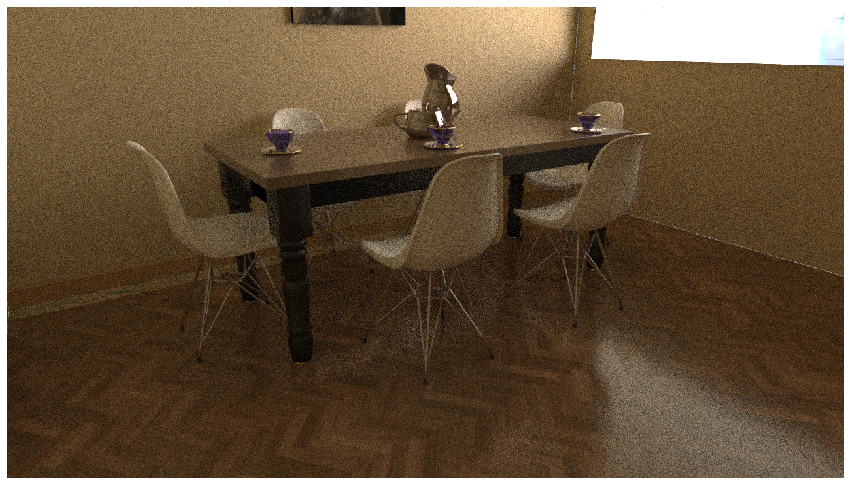
\includegraphics[width=\textwidth]{noisy_color.png}
\caption{Glavni kanal (RGB) uz prisutan šum.}
\label{fig:noisy_color}
\end{figure}

\begin{figure}[H]
\centering
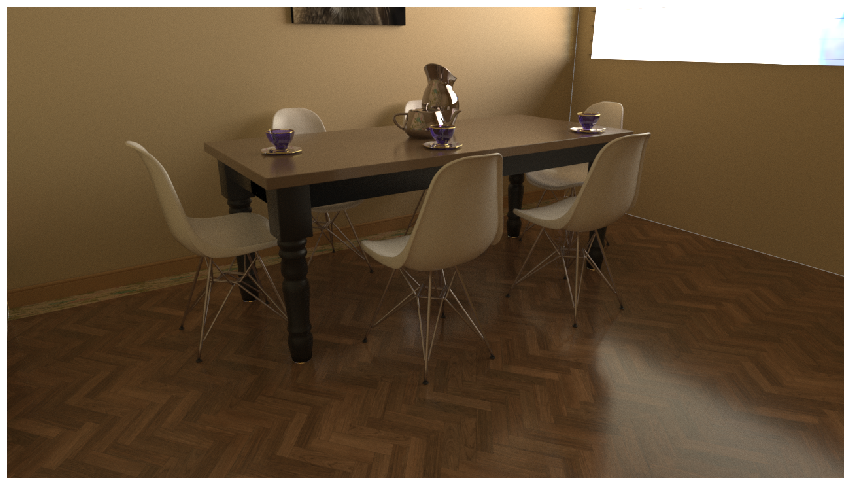
\includegraphics[width=\textwidth]{reference_color.png}
\caption{Glavni kanal (RGB) bez šuma.}
\label{fig:ref_color}
\end{figure}
\end{samepage}

\begin{figure}[H]
\begin{tabular}{cc}
  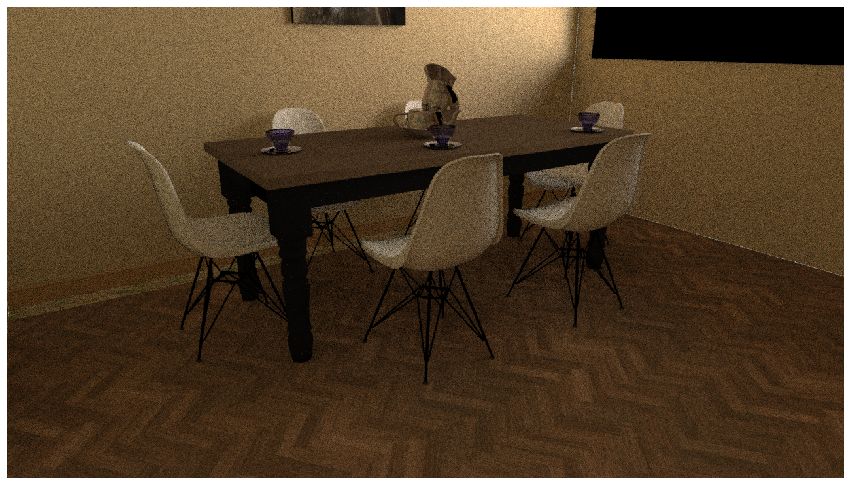
\includegraphics[width=0.5\textwidth]{noisy_diffuse.png} &   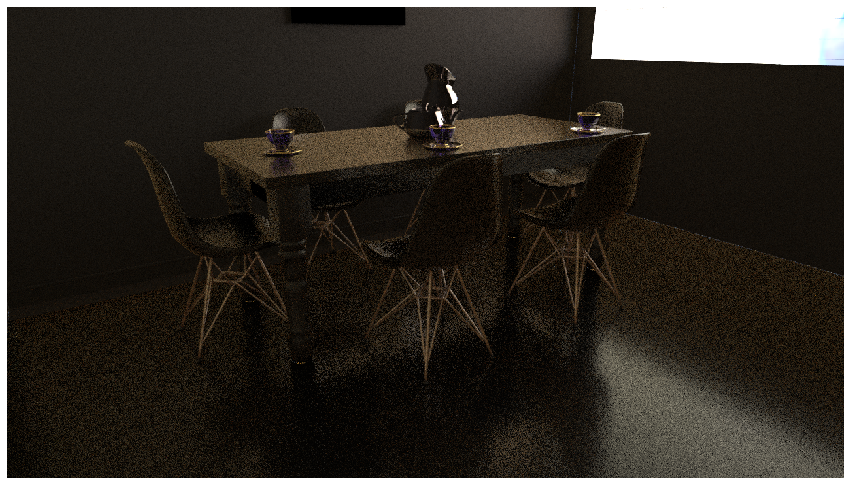
\includegraphics[width=0.5\textwidth]{noisy_specular.png} \\
(a) Difuzna komponenta boje. & (b) Zrcalna komponenta boje. \\[6pt]
 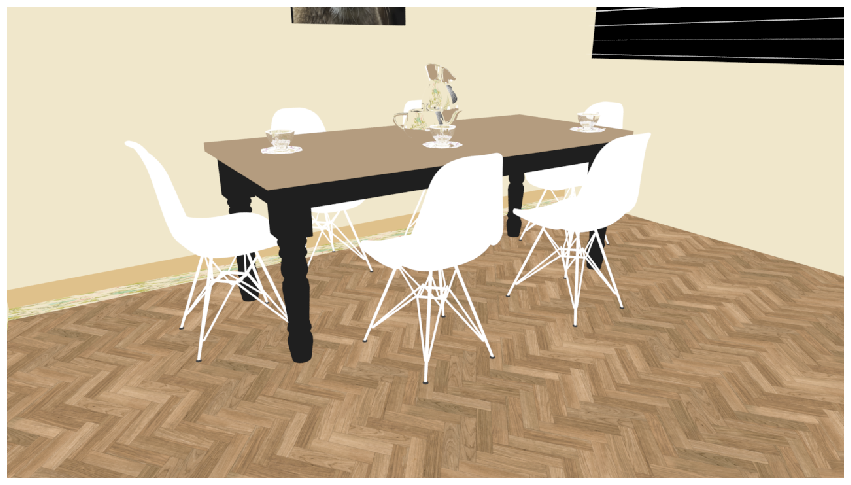
\includegraphics[width=0.5\textwidth]{noisy_albedo.png} &   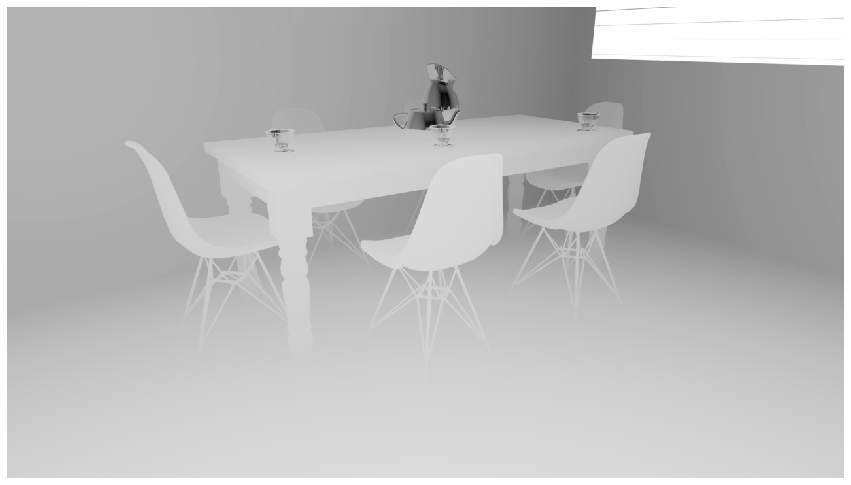
\includegraphics[width=0.5\textwidth]{noisy_depth.png} \\
 (c) Albedo. & (d) Dubina. \\[6pt]
 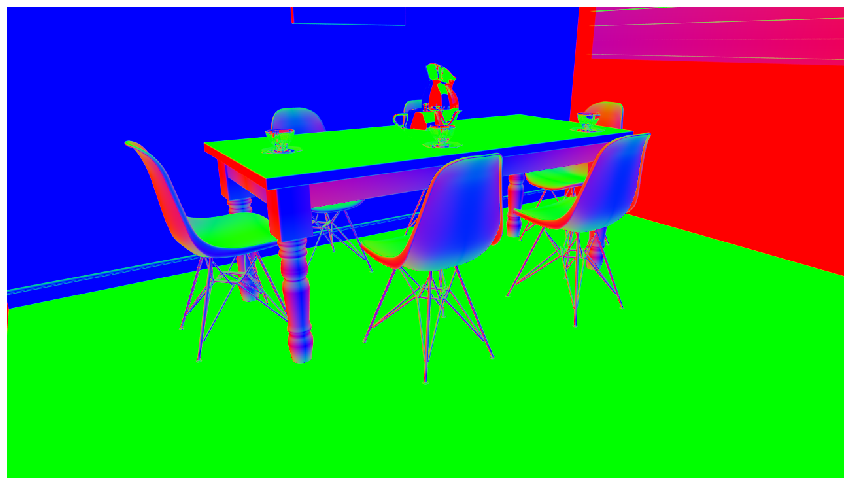
\includegraphics[width=0.5\textwidth]{noisy_normals.png} &   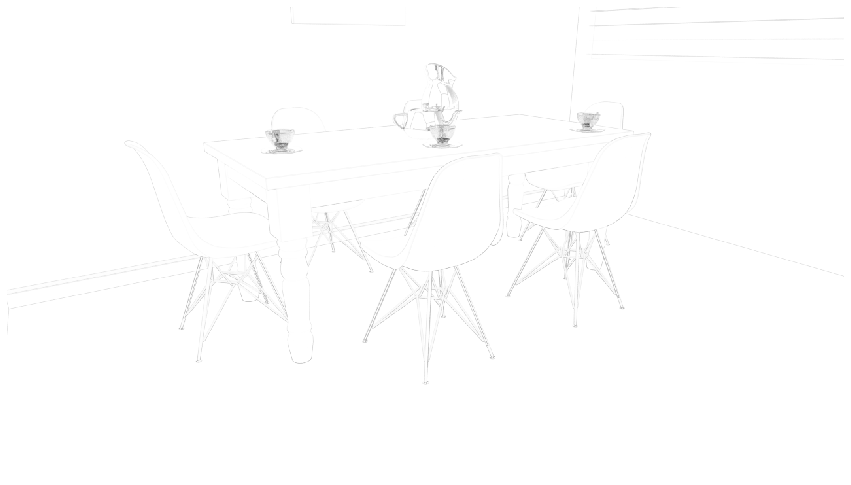
\includegraphics[width=0.5\textwidth]{noisy_normalVariance.png} \\
(e) Normale. & (f) Varijanca normala. \\[6pt]
\end{tabular}
\caption{Dodatne značajke.}
\label{fig:additional_features}
\end{figure}

\section{Pretprocesiranje}
Prije nego krenemo na generiranje parova ulaza i referentnog izlaza, potrebno je obaviti određene
transformacije nad dobivenum slikama.

Difuznu komponentu transformiramo kao
$$ \vect{\tilde{c}}_{\mathrm{diffuse}} = \vect{c}_{\mathrm{diffuse}} \oslash (\vect{f}_{\mathrm{albedo}} + \epsilon), $$
pri čemu je $\oslash$ Hadamardov operator dijeljenja (svaki element lijevog tenzora dijelimo
odgovarajućim elementom desnog tenzora iste veličine), a $\epsilon = 0.00316$ (konstanta iz
članka).

Zrcalnu komponentu ćemo transformirati izrazom
$$ \vect{\tilde{c}}_{\mathrm{specular}} = \log(1 + \vect{c}_{\mathrm{specular}}) $$

Nakon transformiranja ovih dviju komponenti potrebno je transformirati i njihove varijance
sljedećim izrazima:
$$ (\tilde{\sigma}_{\mathrm{diffuse}})^2 \approx \sigma^2_{\mathrm{diffuse}} \oslash
(\vect{f}_{\mathrm{albedo}} + \epsilon)^2, $$
$$ (\tilde{\sigma}_{\mathrm{specular}})^2 \approx \sigma^2_{\mathrm{specular}} \oslash
(\vect{\tilde{c}}_{\mathrm{specular}})^2. $$

Razlog ovih transformacija leži u vrijednostima odgovarajućih komponenti. Difuzna komponenta
inače ima ``pitome'' vrijednosti, ali se u praksi izdvaja albedo kako bi se radilo s efektivnom
osvijetljenošću \engl{effective irradiance}. Ona je glatkija od čiste difuzne komponente i
omogućava nam korištenje jezgri većih dimenzija.

Zrcalna komponenta nam stvara malo više problema. Naime, ona može imati veliki raspon vrijednosti
(i nekoliko redova veličine) i stoga je teško raditi s čistim izlazom te komponente. Zato uvodimo
logaritamsku transformaciju kako bismo dobili manji raspon vrijednosti i osigurali stabilniju
optimizaciju.

Kako bismo iz transformiranih značajki dobili izvorne, potrebno je primijeniti inverzne
transformacije. To je prikazano relacijom
$$ \vect{\hat{c}} = (\vect{f}_{\mathrm{albedo}} + \epsilon) \odot \vect{\hat{c}}_{\mathrm{diffuse}}
+ \exp(\vect{\hat{c}}_{\mathrm{specular}}) - 1, $$
pri čemu su $\vect{\hat{c}}_{\mathrm{diffuse}}$ i $\vect{\hat{c}}_{\mathrm{specular}}$ procjene vrijednosti
odgovarajućih komponenti.

Dodatno, još ćemo izračunati gradijente odgovarajućih kanala u $x$ i $y$ smjerovima, što će
činiti dio ulaza u mrežu. Gradijente računamo tako da od određenog piksela oduzmemo vrijednosti
lijevog ili gornjeg susjeda po svim komponentama. Rubove ćemo popuniti nulama. Funkcije koje
računaju gradijente označavamo s $G_x$ i $G_y$.

\section{Generiranje ulaza neuronske mreže}
Nakon što smo obavili pretprocesiranje, potrebno je generirati sličice \engl{patches} veličine $65\times65$ piksela koje ćemo koristiti kao ulaz u neuronske mreže.

Jedna mogućnost je pozicije sličica odrediti uniformno nasumično, ali to će nam dati puno
``laganih'' primjera s kojih nije teško ukloniti šum (npr. glatka površina). Autori su stoga
odabrali metodu uzorkovanja pomoću mape važnosti \engl{importance map} koja određuje vjerojatnost
odabira sličice s pojedinog područja slike. Ideja je dati veću važnost područjima koja smatramo
težima za postupak uklanjanja šuma kao što su rubovi, nagli prijelazi, velike varijance normala i
boje, itd.

\begin{figure}[h]
\centering
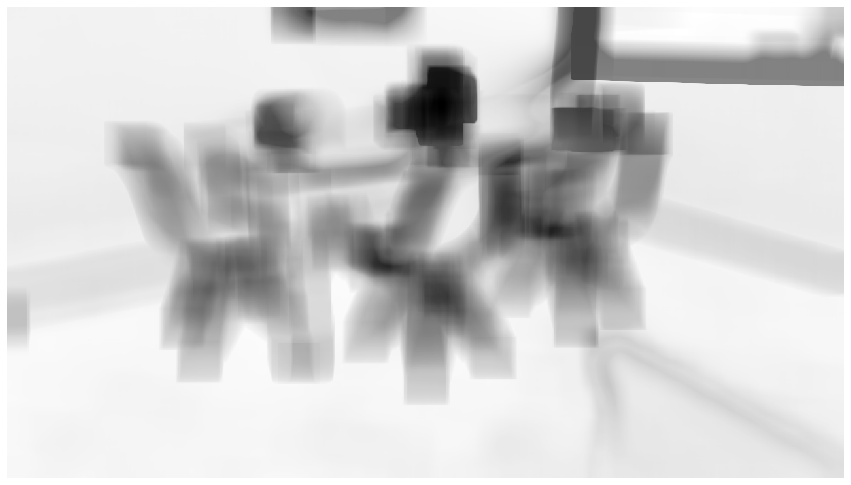
\includegraphics[width=\textwidth]{impmap.png}
\caption{Mapa važnosti za sliku \ref{fig:noisy_color}.}
\label{fig:importance_map}
\end{figure}

Na slici \ref{fig:importance_map} možemo vidjeti primjer mape važnosti. Tamnija područja
označavaju veću važnost, odnosno mjesta gdje očekujemo da će biti teže otkloniti šum i želimo
više primjer s takvih područja. Naravno, ne smijemo zanemariti ostala područja, i ukoliko
određena pozicija bude više puta odbijena zbog male važnosti, automatski ćemo ju dodati u skup.

\begin{figure}
\begin{tabular}{cc}
  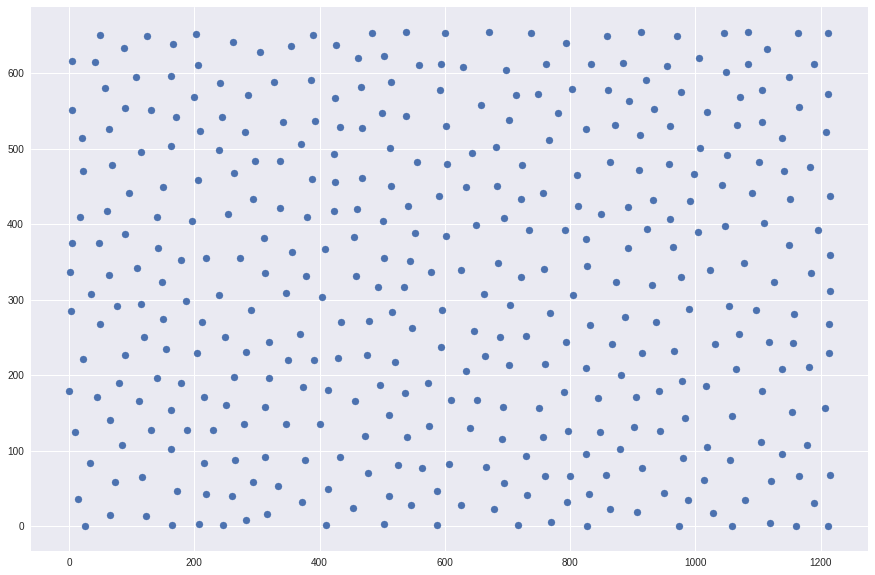
\includegraphics[width=0.5\textwidth]{uniform_patches.png} &   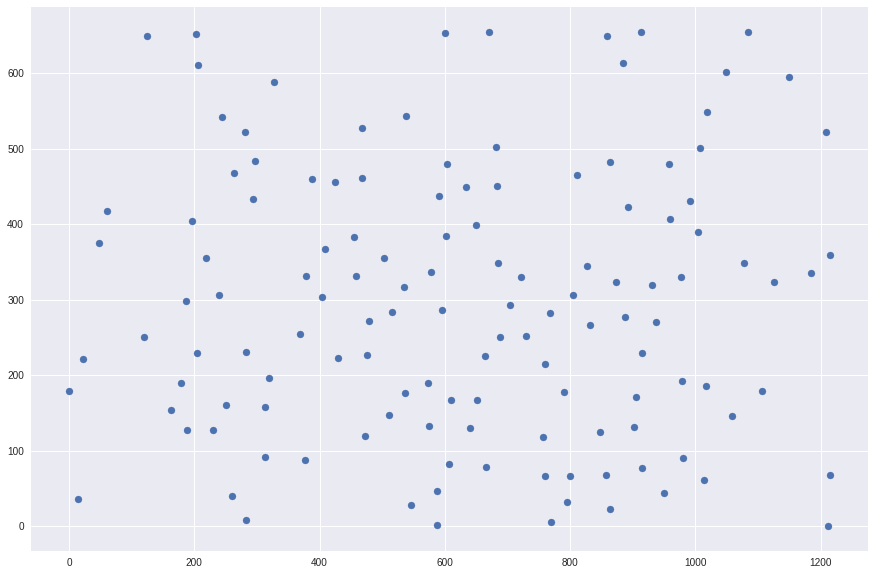
\includegraphics[width=0.5\textwidth]{pruned_patches.png} \\
  (a) Uniformno odabrane pozicije. & (b) Pozicije nakon odbacivanja. \\[6pt]
\end{tabular}
\caption{Odabir pozicija prema mapi važnosti.}
\label{fig:choosing_positions}
\end{figure}

Na slikama \ref{fig:choosing_positions}a i \ref{fig:choosing_positions}b možemo vidjeti utjecaj
mape važnosti. Slika \ref{fig:choosing_positions}a prikazuje početni uniformni odabir pozicija
sličica na velikoj slici. Nakon toga primjenjujemo mapu važnosti i odbacujemo \engl{pruning}
primjere za koje smatramo da neće suviše doprinijeti učenju. Na slici
\ref{fig:choosing_positions}b možemo vidjeti kako je uistinu odabran veći broj primjera s
tamnijih područja mape važnosti, ali je ipak odabrano i mnoštvo primjera sa svjetlijih područja

\begin{samepage}
Nakon što smo obavili pretprocesiranje možemo ``sastaviti'' ulaz u model koji ćemo prikazati kao
$$ \vect{x} = \{ \vect{\tilde{c}}, G_x(\{ \vect{\tilde{c}}, \vect{f} \}),
G_y(\{ \vect{\tilde{c}}, \vect{f} \}), \tilde{\sigma}^2, \tilde{\sigma}^2_{\vect{f}}\}, $$
pri čemu su $G_x$ i $G_y$ gradijenti odgovarajućih značajki u $x$ i $y$ smjeru, a
$\vect{\tilde{c}}$ i $\tilde{\sigma}^2$ mogu pripadati difuznoj ili zrcalnoj komponenti.
\end{samepage}

\begin{figure}[H]
  \centering
  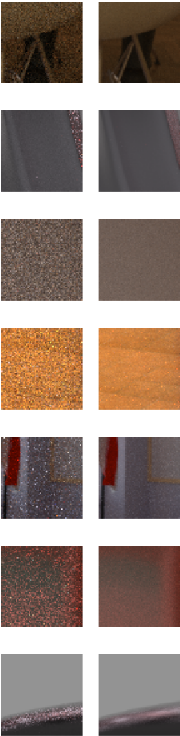
\includegraphics[scale=0.75]{samples_better.png}
  \caption{Primjeri parova odabranih sličica iz skupa za učenje (lijevo ulaz, desno referenca).}
  \label{fig:samples}
\end{figure}


\chapter{Model}
Opisat ćemo dvije varijante modela:
\begin{enumerate}
\item izravna predikcija,
\item predikcija pomoću jezgre.
\end{enumerate}

Obje varijante imaju istu generalnu strukturu, ali se razlikuju u izlazu. Glavni dijelovi su
dvije konvolucijske podmreže koje ćemo zvati difuzna i zrcalna. Jedna podmreža je zadužena za
uklanjanje šuma na difuznoj komponenti, dok je druga zadužena za zrcalnu komponentu boje. Razlog
ovakve podjele leži u različitim karakteristikama tih dviju komponenti--difuzna ima manji raspon
vrijednosti i glatkija je, dok zrcalna komponenta ima veći raspon i drugačiju distribuciju
vrijednosti. Arhitekturu mreže možemo vidjeti na slici \ref{fig:architecture}.

\begin{figure}[H]
  \centering
  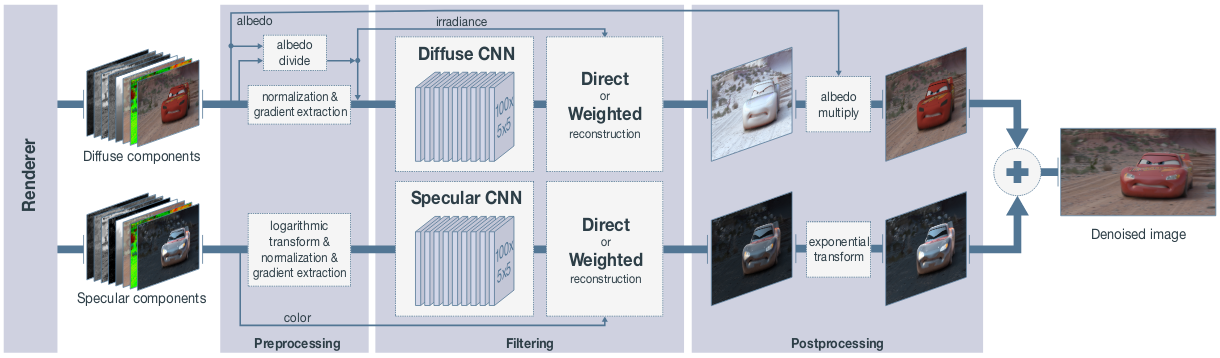
\includegraphics[width=\textwidth]{architecture.png}
  \caption{Arhitektura modela.}
  \label{fig:architecture}
\end{figure}

Konkretnije, podmreže se sastoje od $L$ konvolucijskih slojeva (u našem slučaju $L = 9$), od
kojih svi osim zadnjeg imaju aktivacijsku funkciju ReLU. Nema slojeva sažimanja. Posljednji
sloj nema aktivacijsku funkciju i izlaz mu ovisi o varijanti modela. Također, svaki konvolucijski
sloj osim posljednjeg sadrži $100$ jezgri dimenzija $5\times5$. U nastavku ćemo prvo opisati izravnu predikciju.

\section{Izravna predikcija}
Konvolucijski model s izravnom predikcijom \engl{direct prediction convolutional network, DPCN}
kao izlaz izravno daje predikciju boje piksela bez šuma. Izlaz podmreža je
istih dimenzija kao i slika, a sadrži tri komponente--crvenu, zelenu i plavu. Prednost ove
inačice je jednostavnost, ali se pokazala sporijom za učenje.

Dimenzije tenzora su sljedeće ($B$ je veličina mini grupe, $H$ visina, a $W$ širina slike uz
konvenciju $BCHW$):
\begin{itemize}
\item ulaz: $B \times 28 \times H \times W$,
\item skriveni slojevi: $B \times 100 \times H \times W$,
\item izlaz: $B \times 3 \times H \times W$.
\end{itemize}
Broj parametara iznosi
$$28\times100\times5\times5+100+(L-2)\times(100\times100\times5\times5+100)
+100\times3\times5\times5+3,$$
što za $L=9$ i $k=21$ iznosi $1828303$.

Jedan od problema ove varijante je zamućenje slike \engl{blurring}, što će biti pokazano
u rezultatima. Osim toga, kako nema ograničenja u vrijednostima, model treba više vremena
kako bismo ga istrenirali jer ima veći prostor pretraživanja. To dovodi do pojave artefakata
na slikama.

\section{Predikcija pomoću jezgre}
Druga varijanta modela je konvolucijska mreža s predviđanjem pomoću jezgre
\engl{kernel prediction convolutional network, KPCN}. Ona kao izlaz podmreža daje jezgru
\engl{kernel} za svaki piksel čijom primjenom nad susjedstvom uklanjamo šum sa
središnjeg piksela. Jezgru dobivamo tako da zadnji sloj kao izlaz da onoliko mapi značajki
koliko težina jezgra sadrži.

Dimenzije tenzora su sljedeće ($B$ je veličina mini grupe, $H$ visina, a $W$ širina slike uz
konvenciju $BCHW$):
\begin{itemize}
\item ulaz: $B \times 28 \times H \times W$,
\item skriveni slojevi: $B \times 100 \times H \times W$,
\item izlaz: $B \times k^2 \times H \times W$.
\end{itemize}

Primjerice, u članku je dimenzija jezgre $k = 21$. Tada ćemo na izlazu imati $21^2 = 441$
mapu značajki. Dakle, svaki piksel ima jezgru koju će primijeniti na sebe i svoje susjede, a
ista jezgra se primjenjuje na sve tri RGB komponente.
Broj parametara iznosi
$$28\times100\times5\times5+100+(L-2)\times(100\times100\times5\times5+100)
+100\times k^2\times5\times5+k^2,$$
što za $L=9$ i $k=21$ iznosi $2923741$. To je otprilike $1.6$ puta više parametara od prethodne
varijante.

Dodatno, izlaz se prvo treba ``provući'' kroz aktivacijsku funkciju $\mathrm{Softmax}$ kako bismo
dobili jezgre čije su težine u rasponu $[0, 1]$ i čija je suma jednaka $1$. Razlozi su
višestruki. Kako ova varijanta vuče ideje iz ``klasičnih'' \textit{denoisera},
tako pokušava zadržati dobre aspekte, a popraviti loše (to je uglavnom odabir jezgre). Ono što
postižemo funkcijom $\mathrm{Softmax}$ je sljedeće \cite{Bako2017KPCN}:
\begin{itemize}
\item Osigurava da procjena leži u konveksnoj ljusci susjedstva ulazne slike i time znatno
  smanjuje prostor pretraživanja u odnosu na izravnu predikciju,
\item Osigurava bolje ponašanje gradijenata s obzirom na težine jezgre, tj. treba samo naučiti
  relativnu važnost pojedinog piksela u susjedstvu, a ne mora znati i skalu,
\item Omogućava primjenu na slojeve slike, tako da koristimo jednake težine na svakoj komponenti
  i time osiguravamo da ne dođe do ``pomaka u boji'' i zadržavamo prosječni intenzitet boje \cite{vogels2016thesis}.
\end{itemize}

\section{Učenje modela}

Model treniramo u dva koraka. Prvo treniramo svaku podmrežu zasebno, a zatim
treniramo cijelu mrežu s manjim korakom učenja kako bismo ju fino podesili. Korištenjem mini
grupa pospješujemo generaliziranje mreže i sprječavamo prenaučenost.

Kao algoritam učenja korišten je ADAM, a parametri su inicijalizirani Xavier metodom. Korak učenja
za skup \textit{Tungsten} iznosi $10^{-4}$. Kao funkcija gubitka, korištena je $L_1$ koja računa
apsolutnu razliku između RGB komponenti odgovarajućih piksela. Prilikom učenja, kod konvolucije
nije korišteno nadopunjavanje \engl{padding}.

\chapter{Rezultati}
Usporedimo prvo oba modela po njihovim svojstvima. Model s izravnom predikcijom u nastavku zvat
ćemo DPCN, a model s predikcijom pomoću jezgre zvat ćemo KPCN. Svi eksperimenti su provedeni na
Google Colab GPU instancama.

\section{Usporedba modela}
Podaci su prikazani u tablici \ref{table:comparison}.
\begin{table}[h]
\caption{Usporedba modela}
\begin{center}
\begin{tabular}{ |c|c|c|c| }
\hline
 & DPCN & KPCN \\
\hline
Broj parametara & $1828303$ & $2923741$ \\
Broj slojeva & $9$ & $9$ \\
Veličina izlaza & $B\times3\times H\times W$ & $B\times k^2\times H\times W$ \\
Aktivacijska funkcija na izlazu & - & $\mathrm{Softmax}$\\
\hline
\end{tabular}
\end{center}
\label{table:comparison}
\end{table}

Kao što možemo vidjeti, mreže su vrlo slične, ali KPCN zbog većeg izlaza ima znatno više
parametara. Također, jezgre koje dobijemo na izlazu potrebno je primijeniti na svaki piksel,
odnosno njegovo susjedstvo što nije trivijalna operacija. To model KPCN čini inherentno
sporijim od drugog modela. Autori članka su zbog toga operaciju primjene jezgara implementirali
u jeziku niže razine (C/C++) kao ekstenziju koja se poziva iz biblioteke Tensorflow iz Pythona.

\section{Trajanje učenja modela}
Druga zanimljiva usporedba je potrebno vrijeme učenja između modela. Oba modela mogu doći do iste
pogreške, ali KPCN to čini znatno brže, otprilike 5-6 puta.

Kao eksperiment, provjereno je vrijedi li uistinu tvrdnja da je KPCN brži u učenju od DPCN-a.
Učenje je provedeno na malom podskupu sa stopom učenja $10^{-4}$ u trajanju od 40 epoha.
Rezultat možemo vidjeti na slici \ref{fig:time}.
\begin{figure}[H]
\centering
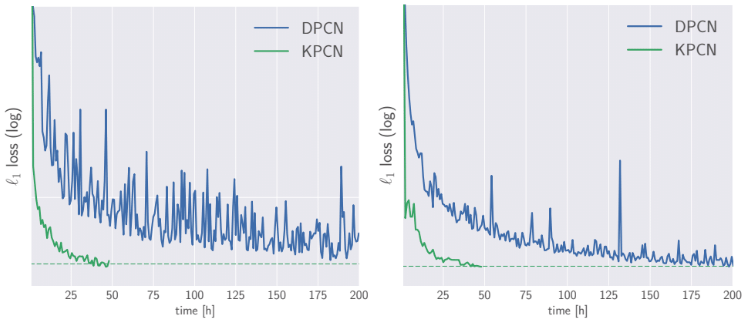
\includegraphics[width=\textwidth]{time.png}
\caption{Usporedba vremena treniranja podmreža (lijevo difuzna, desno zrcalna), preuzeto iz članka
  \cite{Bako2017KPCN}.}
\label{fig:time-paper}
\end{figure}
\begin{figure}[H]
\centering
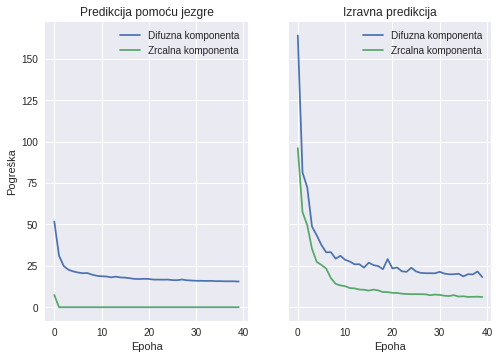
\includegraphics[width=0.7\textwidth]{time_my.png}
\caption{Usporedba vremena učenja difuzne i zrcalne podmreže u oba modela.}
\label{fig:time}
\end{figure}
\begin{figure}[H]
\centering
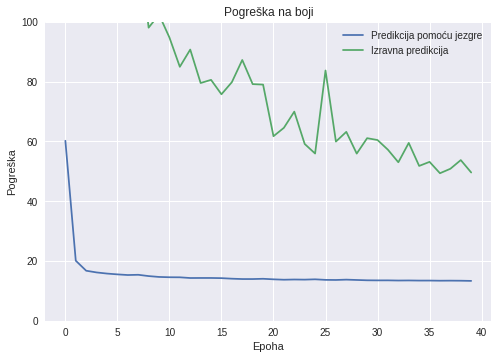
\includegraphics[width=0.7\textwidth]{model_time.png}
\caption{Usporedba vremena učenja krajnjeg izlaza oba modela.}
\label{fig:model-time}
\end{figure}

Prikazani grafovi pokazuju da je KPCN uistinu brži u učenju od konkurenta. Razlog tome je što DPCN
nema ograničenja pa ima mnogo veći prostor pretraživanja. Mora se prilagoditi različitim
rasponima vrijednosti, mora uskladiti RGB komponente kako ne bi došlo do pomaka u boji, itd.
KPCN se ``ogradio'' od toga korištenjem jezgara i funkcije $\mathrm{Softmax}$ što mu omogućava
da prije počne učiti ono glavno--kako ukloniti šum na slici.

Kao dodatna informacija, učenje (40 epoha) DPCN-a je trajalo oko 60 minuta, dok je učenje KPCN-a
trajalo oko 78 minuta što pokazuje kako je aplikacija jezgara prilično zahtjevna operacija.
U vlastitim eksperimentima je implementirana u Pythonu (PyTorch) i nije optimirana kao u
članku.

\section{Primjeri uklanjanja šuma}
Sada ćemo prikazati neke primjere uklanjanja šuma na slikama koje model nije nikada vidio.
Gornja slika je ulaz, srednja izlaz, a donja je referentna.

\begin{figure}[H]
  \centering
\begin{tabular}{cc}
  \multicolumn{2}{c}{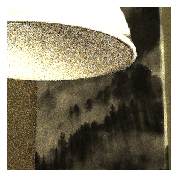
\includegraphics[width=0.3\textwidth]{eval1_in.png}} \\
  \multicolumn{2}{c}{(a) Slika s prisutnim šumom.} \\[6pt]
  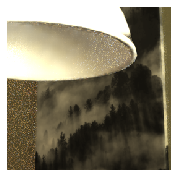
\includegraphics[width=0.3\textwidth]{eval1_kpcn.png} & 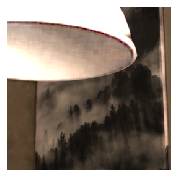
\includegraphics[width=0.3\textwidth]{eval1_dpcn.png} \\
  (b) Izlaz iz KPCN-a. & (c) Izlaz iz DPCN-a. \\[6pt]
  \multicolumn{2}{c}{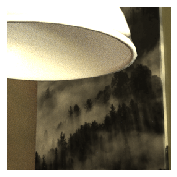
\includegraphics[width=0.3\textwidth]{eval1_ref.png}} \\
  \multicolumn{2}{c}{(d) Referentna slika.} \\[6pt]
\end{tabular}
\caption{Primjer uklanjanja šuma.}
\label{fig:eval1}
\end{figure}
Na slici \ref{fig:eval1}c možemo vidjeti probleme s kojima se DPCN suočava, a to su pomak
u boji i zamućenje. Iako rekonstruirana slika nema vidljiv šum kao na ulaznoj slici, boja
nije onakva kakva bi trebala biti--tamnija je od reference i ulaza. Za razliku, KPCN je
zadržao razinu boje, ali mu je ponegdje ostao vidljiv šum koji bi bio uklonjen treniranjem
na više primjera. Osim toga, rubovi na slici c) nisu oštri kao na ostalim slikama što je
rezultat zamućenja.

\begin{figure}[H]
  \centering
\begin{tabular}{cc}
  \multicolumn{2}{c}{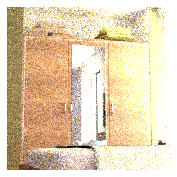
\includegraphics[width=0.3\textwidth]{eval2_in.png}} \\
  \multicolumn{2}{c}{(a) Slika s prisutnim šumom.} \\[6pt]
  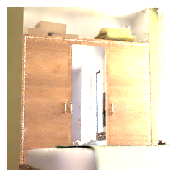
\includegraphics[width=0.3\textwidth]{eval2_kpcn.png} & 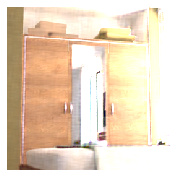
\includegraphics[width=0.3\textwidth]{eval2_dpcn.png} \\
  (b) Izlaz iz KPCN-a. & (c) Izlaz iz DPCN-a. \\[6pt]
  \multicolumn{2}{c}{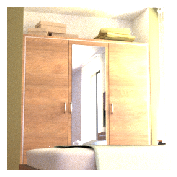
\includegraphics[width=0.3\textwidth]{eval2_ref.png}} \\
  \multicolumn{2}{c}{(d) Referentna slika.} \\[6pt]
\end{tabular}
\caption{Primjer uklanjanja šuma.}
\label{fig:eval2}
\end{figure}

\begin{figure}[H]
  \centering
\begin{tabular}{cc}
  \multicolumn{2}{c}{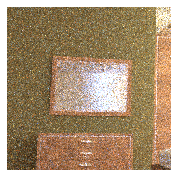
\includegraphics[width=0.3\textwidth]{eval3_in.png}} \\
  \multicolumn{2}{c}{(a) Slika s prisutnim šumom.} \\[6pt]
  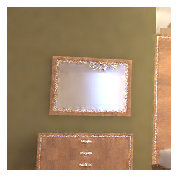
\includegraphics[width=0.3\textwidth]{eval3_kpcn.png} & 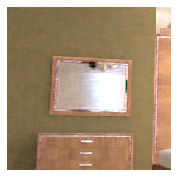
\includegraphics[width=0.3\textwidth]{eval3_dpcn.png} \\
  (b) Izlaz iz KPCN-a. & (c) Izlaz iz DPCN-a. \\[6pt]
  \multicolumn{2}{c}{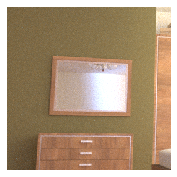
\includegraphics[width=0.3\textwidth]{eval3_ref.png}} \\
  \multicolumn{2}{c}{(d) Referentna slika.} \\[6pt]
\end{tabular}
\caption{Primjer uklanjanja šuma.}
\label{fig:eval3}
\end{figure}
Na slici \ref{fig:eval3}c možemo vidjeti još jedan problem s modelom DPCN, a to je pojava
artefakata (ogledalo). Također, zid ne izgleda glatko i ponovo imamo pomak u boji.

\begin{figure}[H]
  \centering
\begin{tabular}{c}
  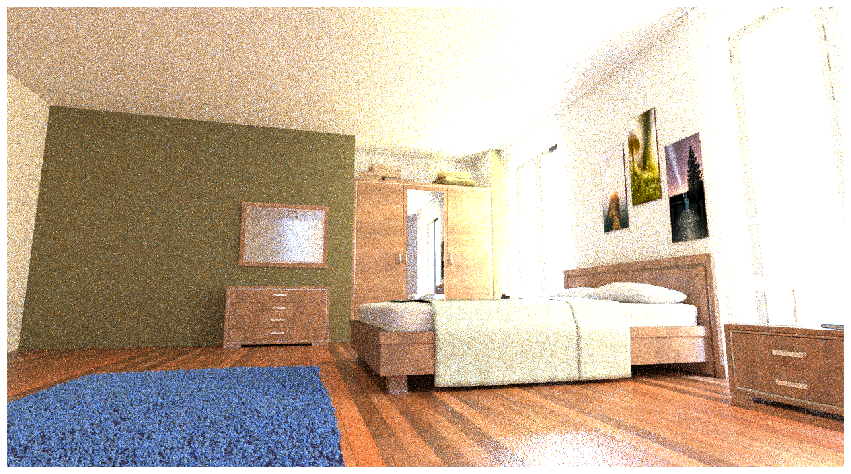
\includegraphics[width=0.75\textwidth]{eval4_in.png} \\
  (a) Slika s prisutnim šumom. \\[6pt]
  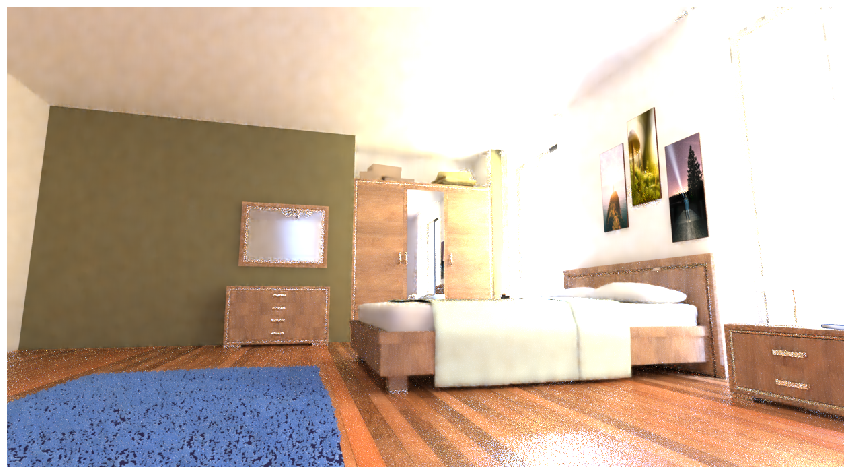
\includegraphics[width=0.75\textwidth]{eval4_kpcn.png} \\
  (b) Izlaz iz KPCN-a. \\[6pt]
  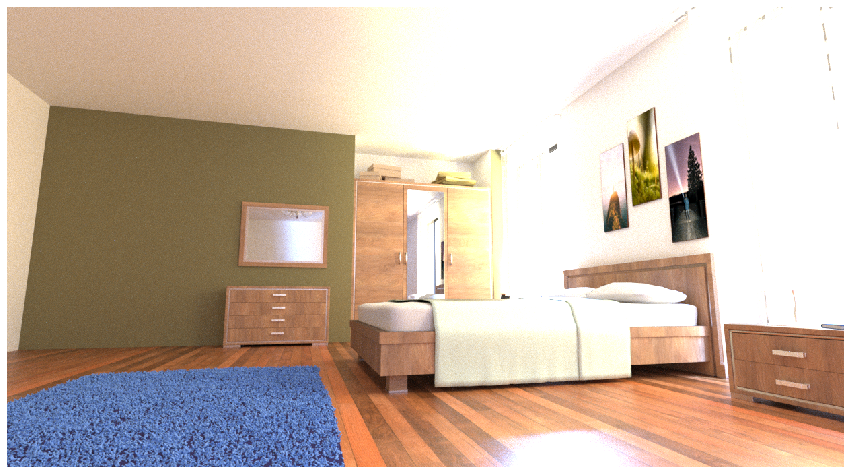
\includegraphics[width=0.75\textwidth]{eval4_ref.png} \\
  (c) Referentna slika. \\[6pt]
\end{tabular}
\caption{Primjer uklanjanja šuma (KPCN).}
\label{fig:eval4kpcn}
\end{figure}

\begin{figure}[H]
  \centering
\begin{tabular}{c}
  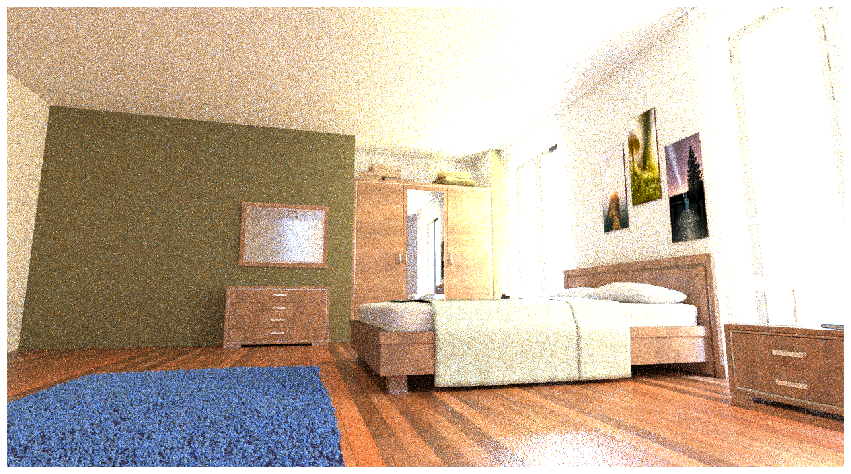
\includegraphics[width=0.75\textwidth]{eval4_in.png} \\
  (a) Slika s prisutnim šumom. \\[6pt]
  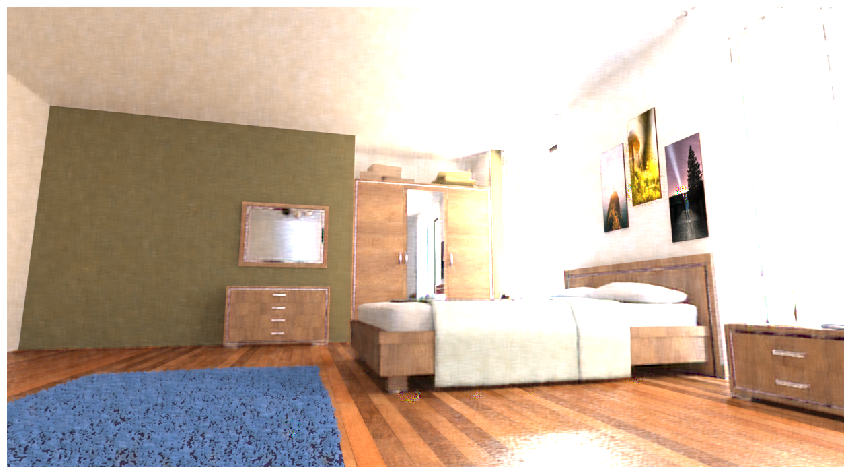
\includegraphics[width=0.75\textwidth]{eval4_dpcn.png} \\
  (b) Izlaz iz DPCN-a. \\[6pt]
  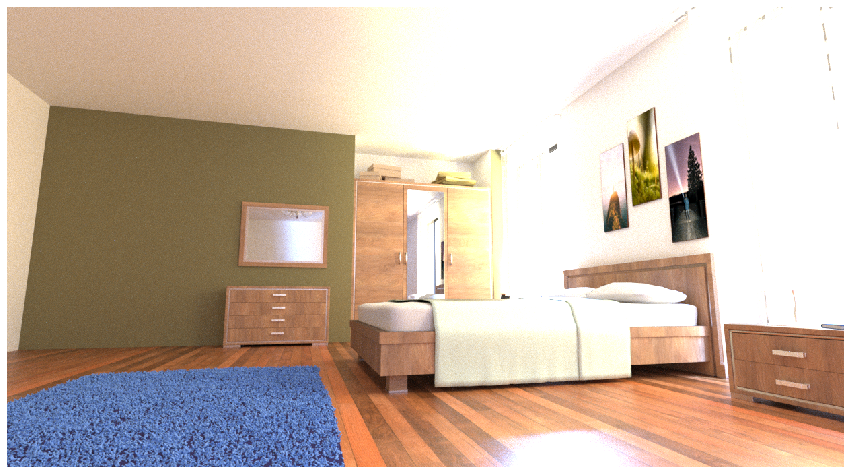
\includegraphics[width=0.75\textwidth]{eval4_ref.png} \\
  (c) Referentna slika. \\[6pt]
\end{tabular}
\caption{Primjer uklanjanja šuma (DPCN).}
\label{fig:eval4dpcn}
\end{figure}

\begin{figure}[H]
  \centering
\begin{tabular}{c}
  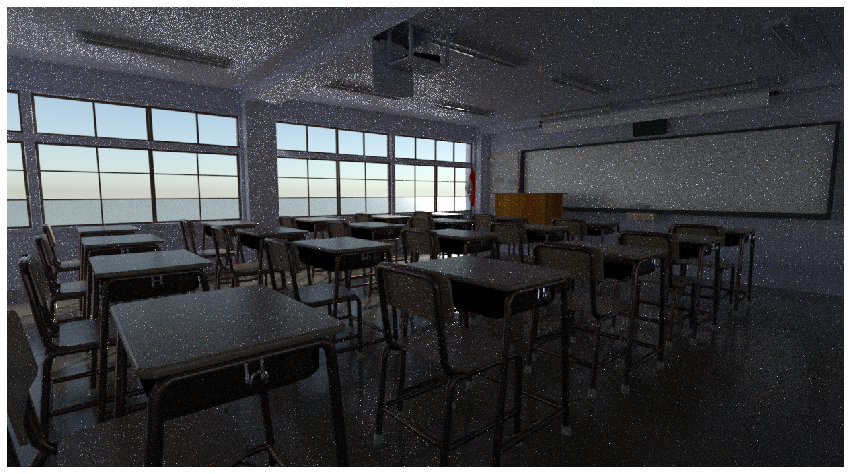
\includegraphics[width=0.75\textwidth]{eval5_in.png} \\
  (a) Slika s prisutnim šumom. \\[6pt]
  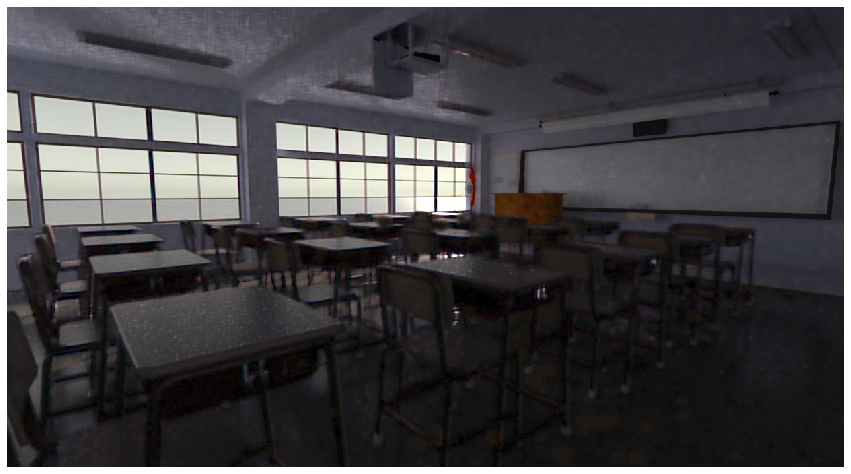
\includegraphics[width=0.75\textwidth]{eval5_dpcn.png} \\
  (b) Izlaz iz DPCN-a. \\[6pt]
  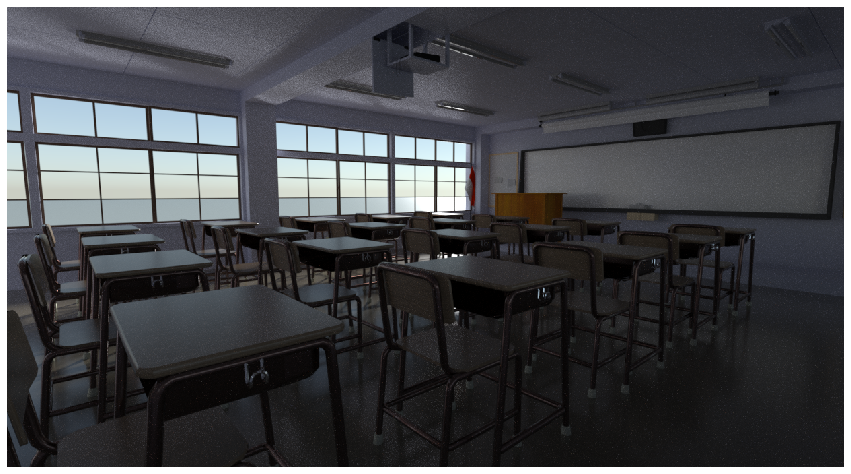
\includegraphics[width=0.75\textwidth]{eval5_ref.png} \\
  (c) Referentna slika. \\[6pt]
\end{tabular}
\caption{Primjer izraženog zamućenja modela DPCN.}
\label{fig:eval5dpcn}
\end{figure}

Većina problema viđenih na slikama bi se mogla popraviti učenjem na većem skupu podataka i
više provedenih epoha. Prikazani rezultati ne koriste cijeli skup za treniranje, već mali
podskup, ali unatoč tome modeli daju prilično dobre rezultate, barem na prvi pogled.

\chapter{Daljnji rad}
Opisana metoda se pokazala odličnom i u trenutku objave je bila \textit{state-of-the-art}.
Ipak, ima određenih nedostataka, a to je primjerice temporalna nestabilnost. Ako bismo ovu
metodu primijenili na nekoliko uzastopnih slika iz animacije, dobili bismo efekt zrnatosti,
odnosno pojavio bi se šum koji možda ne bi bio vidljiv na pojedinoj slici, ali bi došao do
izražaja pri brzoj promjeni između njih.

Osim toga, autori su sugerirali da bi bilo dobro proučiti druge načine odabira sličica za učenje.
Trenutna metoda odabira funkcionira vrlo dobro, ali ima mogućnosti za napredak. Isto vrijedi i za
funkciju gubitka.

Također, bilo bi zanimljivo vidjeti druge pristupe dubokog učenja na ovom problemu,
npr. generativne modele. Paralelno s člankom \cite{Bako2017KPCN} je pisan i
članak\footnote{\url{https://research.nvidia.com/sites/default/files/publications/dnn_denoise_author.pdf}}
u kojemu je naglasak bio na autoenkoderima i većoj interaktivnosti metode (korištenje u
stvarnom vremenu).

\chapter{Tehnički detalji}
Eksperimentiranje je provedeno u programskom jeziku Python verzije 3. Korišten je projekt
Google Colab\footnote{\url{https://colab.research.google.com/}} koji
besplatno nudi vremenski ograničene računalne resurse za potrebe strojnog učenja.
Okolina je Jupyter Python bilježnica koja omogućava interaktivni rad te kombiniranje koda i
teksta. Za manipulaciju EXR datotekama korištena je biblioteka
\texttt{pyexr}\footnote{\url{https://github.com/tvogels/pyexr}} jednog od autora
\cite{Bako2017KPCN}.
Za izradu i učenje neuronskih mreža korišten je računalni okvir
PyTorch\footnote{\url{https://pytorch.org/}} koji se pokazao jako intuitivnim i jednostavnim za
korištenje.
Jupyter bilježnica nalazi se na \href{https://colab.research.google.com/drive/1mz8tbvjPIUbScKTQMPtY7ViRbKOtbg0y}{ovoj adresi}.

\section{Isječci koda}

\begin{lstlisting}[language=Python,
    basicstyle=\tiny,
    caption=Funkcija koja vraća inicijaliziranu podmrežu.]
import torch
import torch.nn as nn
import torch.nn.functional as F

recon_kernel_size = 21

def make_net(n_layers, mode):
  # create first layer manually
  layers = [
      nn.Conv2d(input_channels, hidden_channels, kernel_size),
      nn.ReLU()
  ]

  for l in range(n_layers-2):
    layers += [
        nn.Conv2d(hidden_channels, hidden_channels, kernel_size),
        nn.ReLU()
    ]

  out_channels = 3 if mode == 'DPCN' else recon_kernel_size**2
  layers += [nn.Conv2d(hidden_channels, out_channels, kernel_size)]

  for layer in layers:
    if isinstance(layer, nn.Conv2d):
      nn.init.xavier_uniform_(layer.weight)

  return nn.Sequential(*layers)
\end{lstlisting}


\begin{lstlisting}[language=Python,
    basicstyle=\tiny,
    caption=Funkcije za transformaciju podataka.]
def preprocess_diffuse(diffuse, albedo):
  return diffuse / (albedo + eps)


def postprocess_diffuse(diffuse, albedo):
  return diffuse * (albedo + eps)


def preprocess_specular(specular):
  assert(np.sum(specular < 0) == 0)
  return np.log(specular + 1)


def postprocess_specular(specular):
  return np.exp(specular) - 1


def preprocess_diff_var(variance, albedo):
  return variance / (albedo + eps)**2


def preprocess_spec_var(variance, specular):
  return variance / (specular+1e-5)**2


def gradients(data):
  h, w, c = data.shape
  dX = data[:, 1:, :] - data[:, :w - 1, :]
  dY = data[1:, :, :] - data[:h - 1, :, :]
  # padding with zeros
  dX = np.concatenate((np.zeros([h,1,c], dtype=np.float32),dX), axis=1)
  dY = np.concatenate((np.zeros([1,w,c], dtype=np.float32),dY), axis=0)

  return np.concatenate((dX, dY), axis=2)
\end{lstlisting}

\begin{lstlisting}[language=Python,
    basicstyle=\tiny,
    caption=Kostur postupka učenja podmreža.]
  criterion = nn.L1Loss()

  optimizerDiff = optim.Adam(diffuseNet.parameters(), lr=learning_rate)
  optimizerSpec = optim.Adam(specularNet.parameters(), lr=learning_rate)

  for epoch in range(epochs):
    for i_batch, sample_batched in enumerate(dataloader):
      # get the inputs
      X_diff = sample_batched['X_diff'].permute(permutation).to(device)
      Y_diff = sample_batched['Reference'][:,:,:,:3].permute(permutation).to(device)

      # zero the parameter gradients
      optimizerDiff.zero_grad()

      # forward + backward + optimize
      outputDiff = diffuseNet(X_diff)

      if mode == 'KPCN':
        X_input = crop_like(X_diff, outputDiff)
        outputDiff = apply_kernel(outputDiff, X_input)

      Y_diff = crop_like(Y_diff, outputDiff)

      lossDiff = criterion(outputDiff, Y_diff)
      lossDiff.backward()
      optimizerDiff.step()

      # get the inputs
      X_spec = sample_batched['X_spec'].permute(permutation).to(device)
      Y_spec = sample_batched['Reference'][:,:,:,3:6].permute(permutation).to(device)

      # zero the parameter gradients
      optimizerSpec.zero_grad()

      # forward + backward + optimize
      outputSpec = specularNet(X_spec)

      if mode == 'KPCN':
        X_input = crop_like(X_spec, outputSpec)
        outputSpec = apply_kernel(outputSpec, X_input)

      Y_spec = crop_like(Y_spec, outputSpec)

      lossSpec = criterion(outputSpec, Y_spec)
      lossSpec.backward()
      optimizerSpec.step()

      # calculate final ground truth error
      with torch.no_grad():
        albedo = sample_batched['origAlbedo'].permute(permutation).to(device)
        albedo = crop_like(albedo, outputDiff)

        outputFinal = outputDiff * (albedo + eps) + torch.exp(outputSpec) - 1.0

        Y_final = sample_batched['finalGt'].permute(permutation).to(device)
        Y_final = crop_like(Y_final, outputFinal)

        lossFinal = criterion(outputFinal, Y_final)
\end{lstlisting}

\bibliography{literatura}
\bibliographystyle{fer}

\end{document}
